%%MAIN: thesis.tex

%%%%% The Validation %%%%%
\chapter{Implementation: Lesson Plans} \label{ch_teaching}

In its current form, the ``Processing Abstractions'' environment as presented in chapter \ref{ch_pa} is mainly targetted at the obligatory introduction to computer sciences at high school level.

Before going into empirical results from using this environment in two courses, three lesson plans will be presented for which it has been developed: a \emph{Sichtenwechsel} in computer architecture (section \ref{sc_lesson_ca}); an introduction into the inner workings of a compiler (section \ref{sc_lesson_compiler}); and first a plan for a general introduction to programming (section \ref{sc_lesson_intro}). Some ideas for how to expand it for other school levels will be presented in section \ref{sc_lesson_other}.

For all the lessons, students will need a local environment of ``Processing Abstractions'' installed on a computer available to them. See appendix \ref{app_setup} for how to set it up. Additionally, for non-German speaking students the contents will have to be translated to the teaching language.



\section{Introduction to Programming} \label{sc_lesson_intro}

While the ``Processing Abstractions'' environment has been developed for linking programming and computer architecture, it can also be used for an introduction to programming. This does even help linking programming and computer architecture for students, since they can start at the same point and reuse the experience already gained.


\subsection{Educational objective}

After the introduction, students should ...
\begin{itemize}
\item be able to write programs matching given visual outputs.
\item be able to read and understan programs with a limited command set.
\item be able to learn from their mistakes, correct themselves and not be afraid of breaking things.
\item have a solid foundation for taking on the task of writing a basic but still interesting app or game.
\end{itemize}


\subsection{Prerequisites}

Students need experience in using their own computer, including ...
\begin{itemize}
\item downloading and extracting archives
\item dealing with their virus scanner\footnote{At least under Windows, many scanners flag GT as untrustworthy due to its executable lacking a valid signature. Some virus scanners even block the entire download, if the archive is distributed over a network.}
\end{itemize}


\subsection{Introduction to Glamorous Toolkit} \label{ssc_lesson_gt}

Since Glamorous Toolkit will be a new environment altogether for all students, some basics on its usage have to be introduced first:

\begin{todo}
\item Distribute GT/PA
\item After extracting GT, a brief overview is needed before starting
\item Introduction to GT as an interactive notebook (compare to previously known software such as OneNote or Jupyter)
\item GT is bleeding edge (development on trunk), introduce most pressing issues (navigation, keyboard issues, saving, scrolling, zooming)
\item Some quick tasks for getting the hang of it and identifying students with more supporting needs (let them help themselves)
\item Point more advanced students towards inspectability
\end{todo}


\subsection{Lesson Plans}

\begin{todo}
\item stepwise introduction to Processing (introduced in \ref{sc_processing})
\item imperative, few commands: \texttt{size}, \texttt{rect}, \texttt{ellipse}, \texttt{fill}
\item teaches importance of order
\item tasks: produce given output
\item debugging consists in modifying values (result is immediately visible)
\item quicker and more proficient students can easily skip ahead (loops, animations, recursion)
\item introduce variables, loops, animation, interaction
\item available tools: output, step-by-step debugger (for now, more later)
\end{todo}



\section{Lesson on Computer Architecture} \label{sc_lesson_ca}
% Using PA to demonstrate what happens under the hood when running a program in a high level language.
Introductions to computer science which extend beyond a pure programming course often contain lessons on computer architecture. E.\,g. the curriculum \cite[p.\,145]{Erz16} asks for students to ``know how computers and networks are structured and work''.

Now a sequence of lessons on the subject might be ordered either bottom up (as elaborated in subsection \ref{ssc_bottom_up}) or top down (\ref{ssc_top_down}). In either case, this proposed lesson will go towards the middle or can be used at the end as part of a repetition sequence.

Part of this has been validated (cf. \ref{sc_validation_ca})


\subsection{Educational objective}

\begin{todo}
\item students can explain how a program might actually be run on hardware
\end{todo}


\subsection{Prerequisites}
Students must already know basic programming skills in a high level language such as Processing (see section \ref{sc_processing}). In particular, they must know about variables and loops. An introduction to programming could also be done using \texttt{PA} as outlined in \ref{sc_lesson_intro} above.

The more students are supposed to work on their own, the more they'll need an overview over the different layers prior to combining them. As a prerequisite, it it recommended to at least introduce the Von Neumann architecture and its split of the CPU into control unit and arithmetic unit:

\begin{center}
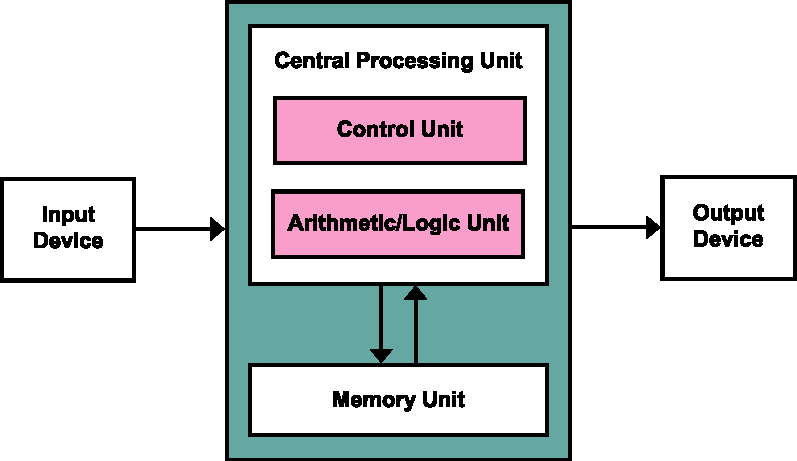
\includegraphics[width=10cm]{images/Von_Neumann_Architecture.pdf}
\\ \xxx{replace or properly attribute: Kapooht, 2013, CC BY-SA 3.0}
\end{center}

In a bottom up approach, this might also include the introduction of transistors, logic gates and circuits. In a top down approach, these could also be treated afterwards.


\subsection{Lesson Plan}

The goal of the lesson is for students to have connected their knowledge of high level programming with what happens within their machine when a program is executed.

If this is the student's encounter with Glamorous Toolkit, at least a brief introduction is in order (see \ref{ssc_lesson_gt}). Else we can directly start with a reminder of what they already know about programming.




\section{Lesson on Compilers} \label{sc_lesson_compiler}

Using PA to demonstrated the steps of lexing, parsing, transpiling, compiling and optimizing.

Part of this has been validated (cf. \ref{sc_validation_compiler})


\subsection{Educational objective}

\begin{todo}
\item students can explain the difference between high and low level language
\item students can enumerate the steps required for compiling a program
\item students have an understanding of the roles a lexer, parser, transpiler and compiler play
\end{todo}


\subsection{Prerequisites}

\begin{todo}
\item programming with Processing (e.\,g. from \ref{sc_lesson_intro})
\item GT/PA installed (e.\,g. from \ref{ssc_lesson_gt})
\item Stacks and registers
\end{todo}


\subsection{Lesson Plan}

\begin{todo}
\item Repetition high level programming (see tasks in PA)
\item Comparision with low level programming (e.\,g. \cite{Tom15}): levels 1 to 6 (introduces jumps, memory access, arithmetic)
\item Presenting/reading overview, compare with natural language
\item Lexer: compare given example with mainly different whitespace; what are tokens?
\item Parser: describe AST in own words, compare with sentence structure from natural languages; develop simple parsing model (\xxx{better views?})
\item Transpiler (optional): compare Processing and Smalltalk
\item Compiler: compare AST with intermediary representation; compare Program with intermediary representation; compare intermediary representation with \cite{Tom15}
\item Optimization: naive examples
\end{todo}



\section{Further Lesson Ideas} \label{sc_lesson_other}

Connecting PA with Smalltalk; extend it to object oriented programming; mould the environment to questions developed during the course; ...
